%%%%%%%%%%%%%%%%%%%%%%%%%%%%%%%%%%%%%%%%%
% Short Sectioned Assignment LaTeX Template Version 1.0 (5/5/12)
% This template has been downloaded from: http://www.LaTeXTemplates.com
% Original author:  Frits Wenneker (http://www.howtotex.com)
% License: CC BY-NC-SA 3.0 (http://creativecommons.org/licenses/by-nc-sa/3.0/)
%%%%%%%%%%%%%%%%%%%%%%%%%%%%%%%%%%%%%%%%%

%----------------------------------------------------------------------------------------
%   PACKAGES AND OTHER DOCUMENT CONFIGURATIONS
%----------------------------------------------------------------------------------------

\documentclass[10pt,a4paper,spanish]{article}

% ---- Entrada y salida de texto -----

\usepackage[spanish]{babel} 
\usepackage[T1]{fontenc} % Use 8-bit encoding that has 256 glyphs
\usepackage[utf8]{inputenc}
\usepackage{minted}
% \usepackage{fourier} % Use the Adobe Utopia font for the document - comment this line to return to the LaTeX default
\usepackage[usenames, dvipsnames]{color}
\usepackage{xcolor}
\usepackage{colortbl}
\usepackage[bookmarks=true,colorlinks=true,linkcolor=red,citecolor=blue]{hyperref}
\usepackage{cite}
\usepackage[official]{eurosym}
\usepackage{tikz}
\usepackage{pgfplots}
\pgfplotsset{compat=1.5}
% \usepackage{pgf-pie}
\usepackage{subfigure}

% ---- Otros paquetes ----
\usepackage{enumerate}
\usepackage{amsmath,amsfonts,amsthm,amssymb} % Math packages
\usepackage{graphics,graphicx} %para incluir imágenes y notas en las imágenes
% Para hacer tablas comlejas
%\usepackage{multirow}
%\usepackage{threeparttable}

\usepackage[a4paper, margin=1.3in]{geometry}


\usepackage{sectsty} % Allows customizing section commands
\allsectionsfont{\centering \normalfont\bfseries\scshape} % Make all sections centered, the default font and small caps

\usepackage{fancyhdr} % Custom headers and footers
\pagestyle{fancyplain} % Makes all pages in the document conform to the custom headers and footers
\fancyhead{} % No page header - if you want one, create it in the same way as the footers below
\fancyfoot[L]{} % Empty left footer
\fancyfoot[C]{} % Empty center footer
\fancyfoot[R]{\thepage} % Page numbering for right footer
\renewcommand{\headrulewidth}{0pt} % Remove header underlines
\renewcommand{\footrulewidth}{0pt} % Remove footer underlines
\setlength{\headheight}{13.6pt} % Customize the height of the header

\numberwithin{equation}{section} % Number equations within sections (i.e. 1.1, 1.2, 2.1, 2.2 instead of 1, 2, 3, 4)
\numberwithin{figure}{section} % Number figures within sections (i.e. 1.1, 1.2, 2.1, 2.2 instead of 1, 2, 3, 4)
\numberwithin{table}{section} % Number tables within sections (i.e. 1.1, 1.2, 2.1, 2.2 instead of 1, 2, 3, 4)

\setlength\parindent{0pt} % Removes all indentation from paragraphs - comment this line for an assignment with lots of text
\setlength{\parskip}{1ex plus 0.5ex minus 0.2ex}

\newcommand{\horrule}[1]{\rule{\linewidth}{#1}} % Create horizontal rule command with 1 argument of height

%----------------------------------------------------------------------------------------
%   TÍTULO Y DATOS DEL ALUMNO
%----------------------------------------------------------------------------------------

\title{
\normalfont \normalsize 
\textsc{{\bf Ingeniería de Servidores (2015-2016)} \\ Grado en Ingeniería Informática \\ Universidad de Granada} \\ [25pt] % Your university, school and/or department name(s)
\horrule{0.5pt} \\[0.4cm] % Thin top horizontal rule
\huge Memoria Práctica 4 \\ % The assignment title
\horrule{2pt} \\[0.5cm] % Thick bottom horizontal rule
}

\author{Marta Gómez Macías} % Nombre y apellidos

\date{\normalsize\today} % Incluye la fecha actual

\newmintedfile[mybash]{bash}{
    linenos,
    numbersep=5pt,
    gobble=0,
    frame=lines,
    framesep=2mm,
    tabsize=3,
}

\newmintedfile[myyml]{yaml}{
    linenos,
    numbersep=5pt,
    gobble=0,
    frame=lines,
    framesep=2mm,
    tabsize=3,
}

\newmintedfile[mypython]{python}{
    linenos,
    numbersep=5pt,
    gobble=0,
    frame=lines,
    framesep=2mm,
    tabsize=3,
}

%----------------------------------------------------------------------------------------
% DOCUMENTO
%----------------------------------------------------------------------------------------

\begin{document}
%Cambiar Cuadros por Tablas y lista de...
\renewcommand{\listtablename}{Índice de tablas}
% \renewcommand{\tablename}{Tabla} 

\maketitle % Muestra el Título
\pagenumbering{gobble} 

\newpage %inserta un salto de página
\pagenumbering{arabic} 

\tableofcontents % para generar el índice de contenidos

\listoffigures

% \listoftables

\newpage

\section{Instale la aplicación \textit{Phoronix}. ¿Qué comando permite listar los benchmarks disponibles?}
En \cite{phoronixubuntu} encontramos una pequeña guía tanto de instalación como de uso de \textit{Phoronix}. Para instalar el benchmark en Ubuntu sólo nos basta con usar el siguiente comando:
\begin{minted}[frame=single, label={Instalando phoronix-test-suite en Ubuntu}]{bash}
sudo apt-get install phoronix-test-suite
\end{minted}

En \textit{Phoronix} tenemos por un lado las \textit{suites} y por otro lado los \textit{test}. Las suites son grupos de \textit{test} y los \textit{test} son pruebas individuales, en el enunciado de la práctica se mencionan como \textbf{\textit{benchmarks}}.

Para ver las \textit{suites} disponibles usamos el comando:
\begin{minted}[frame=single, label={Listando las suites disponibles para Phoronix}]{bash}
phoronix-test-suite list-available-suites
\end{minted}

Al ejecutar el comando por primera vez nos preguntará varias cosas tales como si aceptamos la licencia o permitimos que se envíen datos a los servidores de \textit{Phoronix}, tras aceptar, empezarán a aparecer en pantalla distintas \textit{suites} poco a poco. 

En la \hyperref[suitesdisponibles]{Figura \ref*{suitesdisponibles}} vemos un ejemplo de output de este comando (sin las preguntas que nos muestra por primera vez) donde vemos algunas \textit{suites} interesantes tales como una \textit{suite} de \textit{gaming}, otra de una base de datos, etc.

\begin{figure}[!h]
    \centering
    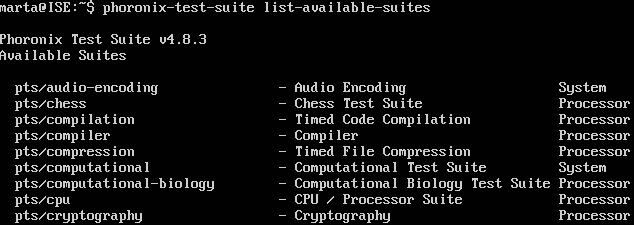
\includegraphics[width=0.9\textwidth]{1}
    \caption{Algunas de las suites disponibles para \textit{Phoronix}}
    \label{suitesdisponibles}
\end{figure}

Para listar los \textit{test} disponibles usamos el comando:
\begin{minted}[frame=single, label={Listando los test disponibles para Phoronix}]{bash}
phoronix-test-suite list-available-tests
\end{minted}

Donde obtendremos una salida bastante parecida a la obtenida con el comando para listar listar las \textit{suites} disponibles (\hyperref[testsdisponibles]{Figura \ref*{testsdisponibles}}). Con la diferencia de que la salida será mucho más rápida.

\begin{figure}[!h]
    \centering
    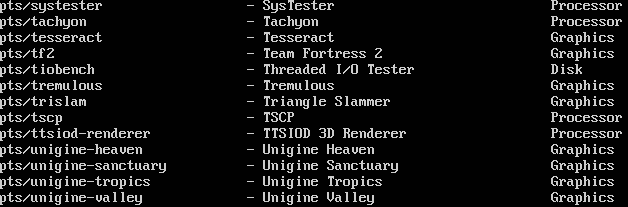
\includegraphics[width=0.9\textwidth]{2}
    \caption{Algunos de los benchmarks disponibles para \textit{Phoronix}}
    \label{testsdisponibles}
\end{figure}

\section{De los parámetros que que podemos pasar al comando ¿Qué significa \texttt{-c 5}? ¿y \texttt{-n 100}? Monitorice la ejecución de \texttt{ab} contra alguna máquina (cualquiera) ¿cuántos procesos o hebras crea \texttt{ab} en el cliente?}
Según \cite{ab}, la opción \texttt{-c} especifica el número de peticiones que se hacen al servidor a la vez concurrentemente. Por defecto su valor es 1. Si su valor es mayor a 1, \texttt{ab} creará en el cliente tantos procesos concurrentes como se establezca en dicho valor, por tanto, en nuestro ejemplo, \texttt{ab} creará 5 procesos concurrentes.

La opción \texttt{-n} especifica el número de peticiones que se hacen para la sesión de benchmarking, el valor por defecto es 1 y normalmente no suele dar resultados representativos.

Para ejecutar el benchmark en un cliente sobre un servidor Apache, ejecutamos el siguiente comando:
\begin{minted}[frame=single, label={Ejecutando Apache Benchmark sobre un servidor}]{bash}
ab -c 5 -n 100 http://10.0.2.10/
\end{minted}

También podríamos hacerlo sobre nuestra propia máquina cambiando la dirección IP del servidor por \texttt{http://localhost/}.

La salida obtenida tras ejecutar \texttt{ab} se ve en la \hyperref[ab]{Figura \ref*{ab}}. En primer lugar nos muestra información sobre el servidor al que le ejecutamos el benchmark. Después, nos muestra información sobre el documento HTML con el que va a trabajar el benchmark para hacer las pruebas. A continuación, nos muestra datos sobre el benchmark tales como nivel de concurrencia, tiempo total de ejecución, peticiones completadas y fallidas, etc. Como se esperaba, el nivel de concurrencia ha sido 5 y el número de peticiones, 100. Por último, nos muestra resultados estadísticos a modo de resumen sobre las 100 peticiones que hemos hecho: el máximo tiempo empleado para servir el \textit{index.html} han sido 20 ms y el mínimo, 3. De las 100 peticiones hechas, el 50\% ha tardado menos de 6ms en ser respondidas.

\begin{figure}[H]
    \centering
    
    \mbox {
        \subfigure[Primera parte del output obtenido tras ejecutar \texttt{ab}]{
        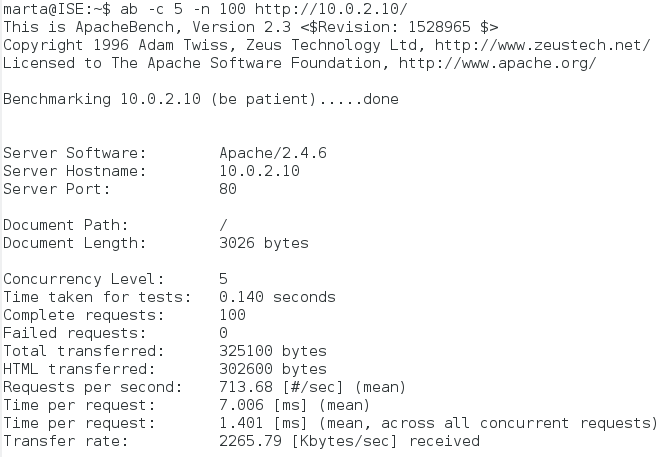
\includegraphics[width=0.55\textwidth]{4}
        \label{ab1}
    }
    \qquad
    
    \subfigure[Segunda parte del output obtenido tras ejecutar \texttt{ab}] {
        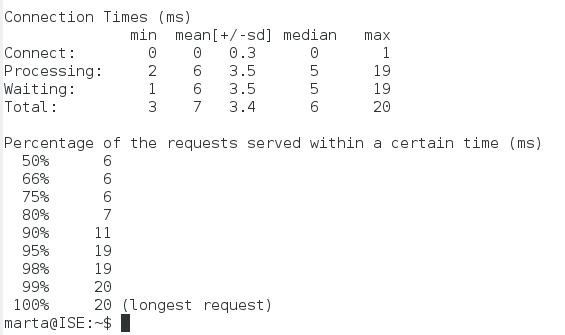
\includegraphics[width=0.55\textwidth]{5}
        \label{ab2}
        }
    }
    \caption{Output obtenido tras ejecutar \texttt{ab}}
    \label{ab}
\end{figure}

\section{Ejecute \texttt{ab} contra las tres máquinas virtuales (desde el SO anfitrión a las máquinas virtuales de la red local) una a una (arrancadas por separado) y muestre y comente las estadísticas. ¿Cuál es la que proporciona mejores resultados? Fíjese en el número de bytes transferidos, ¿es igual para cada máquina?}

Es imposible que el número de bytes transferidos sea igual para cada máquina pues cada una tiene un fichero \textit{index.html} diferente. Para que fuera el mismo tamaño en todas deberíamos eliminar la página de inicio por defecto y poner la misma en todos los servidores.

En el caso de Ubuntu, hemos obtenido los resultados que se ven en la \hyperref[abubuntu]{Figura \ref*{abubuntu}}. La longitud del documento en este caso ha sido de 11510 bytes y la respuesta más lenta se ha hecho en 68 ms.

\begin{figure}[!h]
    \centering
    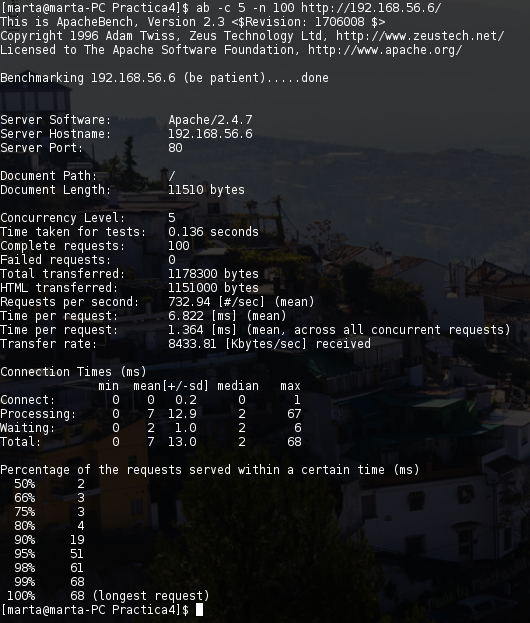
\includegraphics[width=0.7\textwidth]{6}
    \caption{Salida obtenida tras ejecutar \texttt{ab} contra el servidor con Ubuntu Server}
    \label{abubuntu}
\end{figure}

En el caso de CentOS, hemos obtenido los resultados que se ven en la \hyperref[abcentos]{Figura \ref*{abcentos}}. La longitud del documento ha sido de 3026 bytes y la respuesta más lento se ha hecho en 745 ms. Siendo el archivo a transferir de un tamaño inferior, la respuesta ha sido muchísimo más lenta que en el caso del servidor con Ubuntu Server.

\begin{figure}[!h]
    \centering
    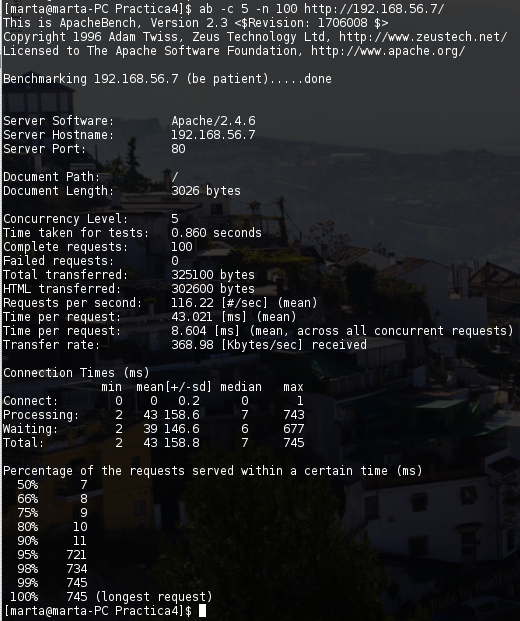
\includegraphics[width=0.7\textwidth]{7}
    \caption{Salida obtenida tras ejecutar \texttt{ab} contra el servidor con CentOS}
    \label{abcentos}
\end{figure}

Por último, en el caso de Windows Server, hemos obtenido los resultados que se ven en la \hyperref[abwindows]{Figura \ref*{abwindows}}. La longitud del documento ha sido de 689 bytes y la respuesta más lenta se ha realizado en más de un segundo. Teniendo que transferir un archivo que pesa menos de 1KB pienso que esta es la máquina más lenta de las tres. 

\begin{figure}[!h]
    \centering
    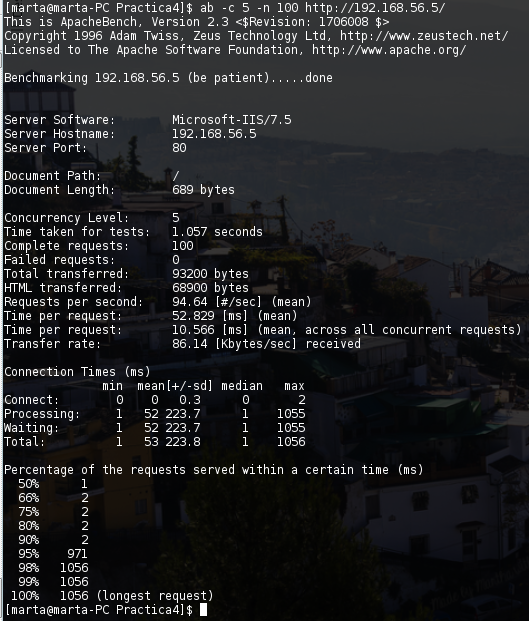
\includegraphics[width=0.7\textwidth]{8}
    \caption{Salida obtenida tras ejecutar \texttt{ab} contra el servidor con Windows Server}
    \label{abwindows}
\end{figure}

Si tuviésemos que hacer un ``ranking'', cuya puntuación se obtendría con la parte entera de la división del tamaño del documento entre el tiempo de respuesta máximo, Ubuntu quedaría en primer puesto con 169 puntos, le seguiría CentOS con 4 y por último estaría Windows Server con 0.

\section{Instale \textit{jmeter} y siga el tutorial para hacer un \textit{Web Test Plan} realizando capturas de pantalla y comentándolas. En vez de usar la web de \textit{jmeter}, haga el experimento usando alguna de sus máquinas virtuales (puede hacer una página sencilla, usar las páginas de phpmyadmin, instalar un CMS, etc)}
\subsection{Instalando \textit{jmeter}}
En primer lugar, debemos descargar el fichero ejecutable de \textit{jmeter}. Para ello, usamos el siguiente comando:

\begin{minted}[frame=single, label={Descargando el ejecutable de jmeter}]{bash}
wget http://apache.rediris.es//jmeter/binaries/apache-jmeter-2.13.tgz
\end{minted}

Tras ello, nos descargamos el fichero \textit{MD5}, para así verificar que no nos hemos descargado ningún \textit{jmeter} ``modificado'':
\begin{minted}[frame=single, label={Descargando el fichero MD5 de jmeter}]{bash}
wget https://www.apache.org/dist/jmeter/binaries/apache-jmeter-2.13.tgz.md5
\end{minted}

Para verificarlo, según \cite{md5apache}, usamos el siguiente comando:
\begin{minted}[frame=single, label={Verificando la descarga de jmeter}]{bash}
md5sum -c apache-jmeter-2.13.tgz.md5
\end{minted}

Si todo ha ido bien, debemos ver un mensaje diciendonos que la suma coincide.

Descomprimimos el archivo descargado, para ello, según \cite{tar}, usamos el siguiente comando:
\begin{minted}[frame=single, label={Descomprimiendo el archivo descargado}]{bash}
tar zxvf apache-jmeter-2.13.tgz
\end{minted}

Tras descomprimir el archivo, vamos al directorio extraído y abrimos el archivo llamado \textit{README} en el que encontraremos las instrucciones de instalación. Que básicamente consisten en irse al directorio \textit{bin} y ejecutar el archivo \texttt{jmeter}:

\begin{minted}[frame=single, label={Pasos para ejecutar jmeter una vez extraído el archivo tgz}, linenos]{console}
$ cd apache-jmeter-2.13/
$ cat README
$ cd bin/
$ ./jmeter
\end{minted}

Tras esto, se nos abrirá la ventana que se ve en la \hyperref[jmeter]{Figura \ref*{jmeter}}.

\begin{figure}[!h]
    \centering
    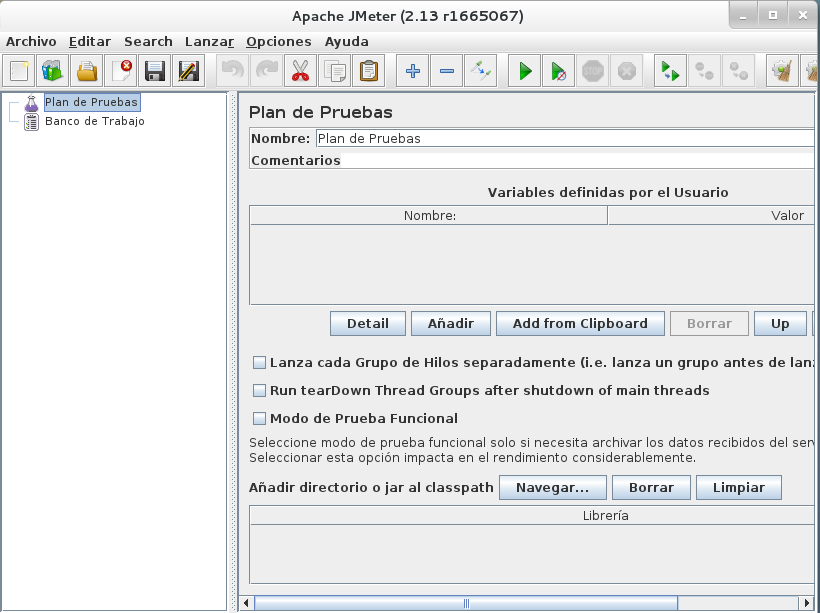
\includegraphics[width=0.7\textwidth]{9}
    \caption{Ventana inicial de \textit{jmeter}}
    \label{jmeter}
\end{figure}

\subsection{Construyendo nuestro propio \textit{Web Test Plan}}
Los pasos a seguir, según \cite{apachetuto}, son:
\begin{enumerate}[1.]
    \item En primer lugar, añadimos un \textit{Grupo de hilos} para poder simular el número de usuarios, la frecuencia con la que mandarán solicitudes y cuántas solicitudes mandarán. Para ello, seguimos la ruta \textbf{Editar $>$ Hilos (Usuarios) $>$ Grupo de Hilos} (\hyperref[grupohilos]{Figura \ref*{grupohilos}}).

    \begin{figure}[!h]
        \centering
        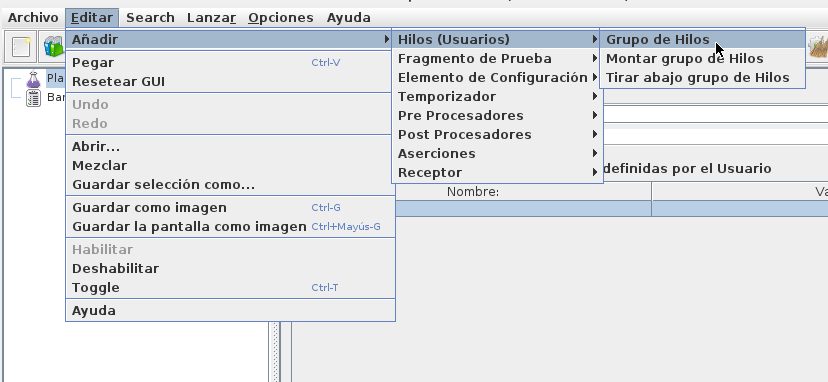
\includegraphics[width=0.5\textwidth]{10}
        \caption{Ruta para crear un \textit{Grupo de hilos}}
        \label{grupohilos}
    \end{figure}

    \item Tras esto, se nos abrirá una ventana en la cual podremos modificar las propiedades del \textit{Grupo de Hilos por defecto}. En nuestro caso serán las que se ven en la \hyperref[grupohilospro]{Figura \ref*{grupohilospro}}: tendremos 5 usuarios mandando peticiones, todos los usuarios se crearán en 1 segundo (es decir, cada usuario tardará en crearse la quinta parte de un segundo) y repetiremos el test dos veces.

    \begin{figure}[!h]
        \centering
        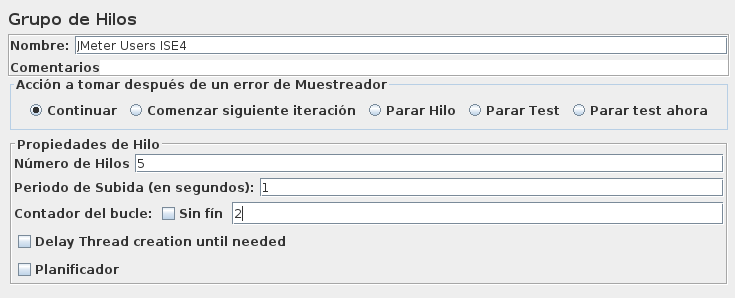
\includegraphics[width=0.5\textwidth]{11}
        \caption{Propiedades para el grupo de hilos que usaremos como ejemplo}
        \label{grupohilospro}
    \end{figure}

    \item Una vez definidos los usuarios, debemos definir lo que harán. Para ello, especificaremos cómo serán las peticiones HTTP. Para ello hacemos click derecho en el \textit{Grupo de Hilos} creado y seguimos la ruta \textbf{Añadir $>$ Elemento de Configuración $>$ Valores por Defecto para Petición HTTP} (\hyperref[peticionhttp]{Figura \ref*{peticionhttp}}).

    \begin{figure}[!h]
        \centering
        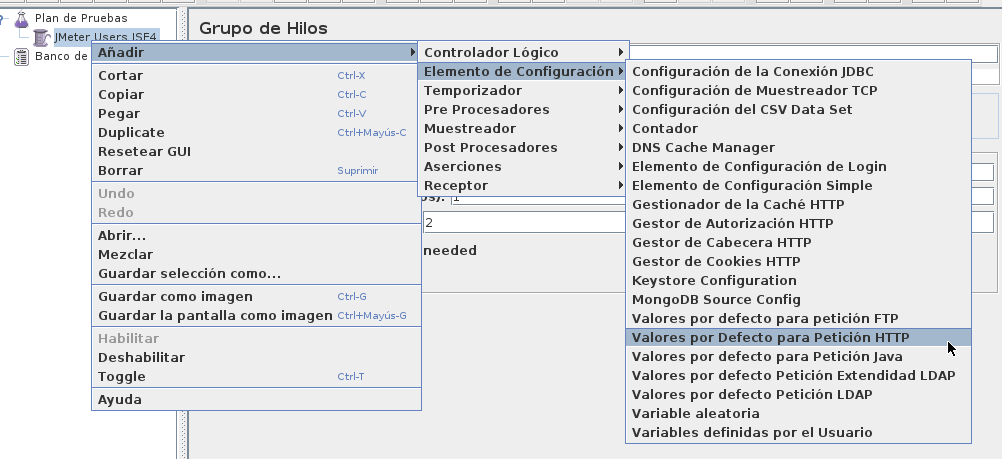
\includegraphics[width=0.5\textwidth]{12}
        \caption{Ruta a seguir para especificar los valores por defecto de una petición HTTP para un grupo de hilos concreto}
        \label{peticionhttp}
    \end{figure}

    \item En este caso, vamos a dejar todos los valores por defecto y, en vez de introducir el servidor de \textit{jmeter}, introduciremos el que tenemos instalado en Ubuntu Server (\texttt{10.0.2.9}). Así, nos debe quedar tal y como se ve en la \hyperref[defaulthttp]{Figura \ref*{defaulthttp}}.

    \begin{figure}[!h]
        \centering
        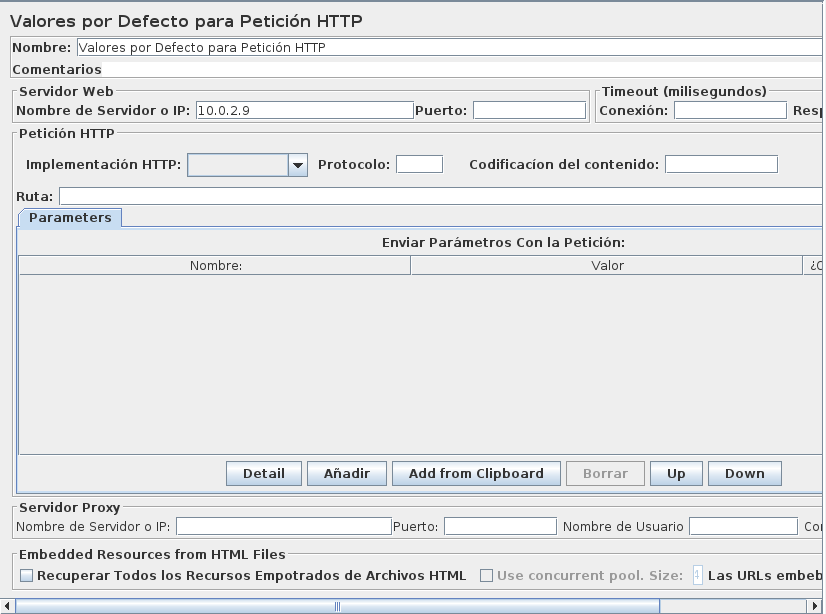
\includegraphics[width=0.5\textwidth]{13}
        \caption{Propiedades para las peticiones HTTP a simular}
        \label{defaulthttp}
    \end{figure}

    \item Opcionalmente, podemos añadir cookies a nuestro \textit{test plan}. Para ello, hacemos click derecho en el \textit{Grupo de hilos} creado y seguimos la ruta \textbf{Añadir $>$ Elemento de configuración $>$ Gestor de Cookies HTTP}. (\hyperref[rutacookies]{Figura \ref*{rutacookies}}). Dejamos todos los valores por defeco en la ventana que obtendremos (\hyperref[gestorcookies]{Figura \ref*{gestorcookies}}).

    \begin{figure}[H]
        \centering
        
        \mbox {
            \subfigure[Ruta a seguir para añadir cookies a nuestro \textit{test plan}]{
            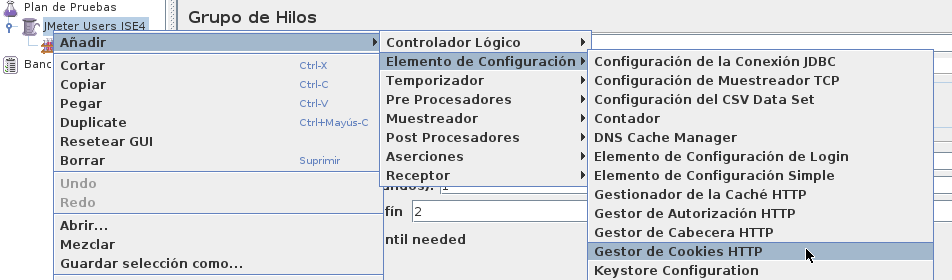
\includegraphics[width=0.55\textwidth]{14}
            \label{rutacookies}
        }
        \qquad
        
        \subfigure[Ventana del gestor de cookies] {
            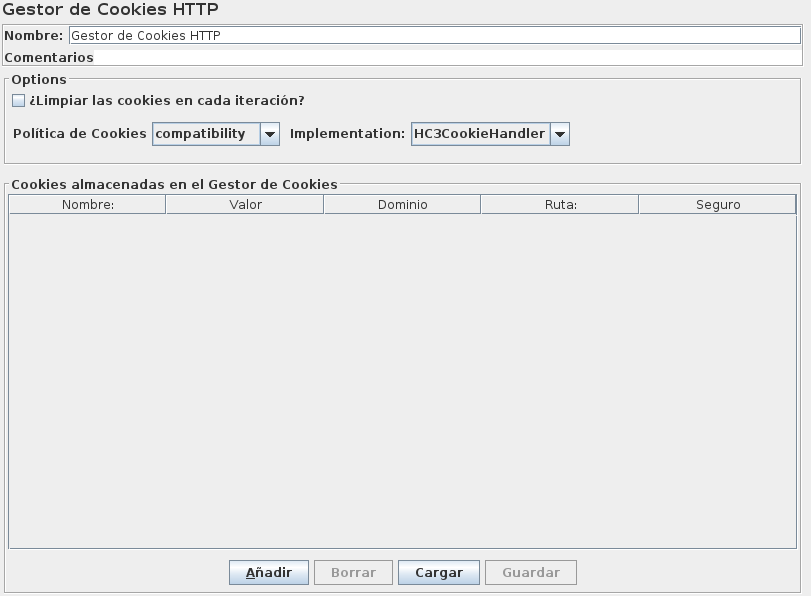
\includegraphics[width=0.55\textwidth]{15}
            \label{gestorcookies}
            }
        }
        \caption{Añadiendo soporte para cookies a nuestro \textit{test plan}}
        \label{galletas}
    \end{figure}   

    \item Ahora añadiremos las peticiones HTTP. Como en nuestro caso sólo tenemos una página de inicio (la que trae por defecto el servidor apache en Ubuntu), añadiremos sólo una petición HTTP a nuestra página de inicio. Para ello, hacemos click derecho en nuestro \textit{Grupo de Hilos} y seguimos la ruta \textbf{Añadir $>$ Muestreador $>$ Petición HTTP}. (\hyperref[rutapethtt]{Figura \ref*{rutapethtt}}).

    \begin{figure}[!h]
        \centering
        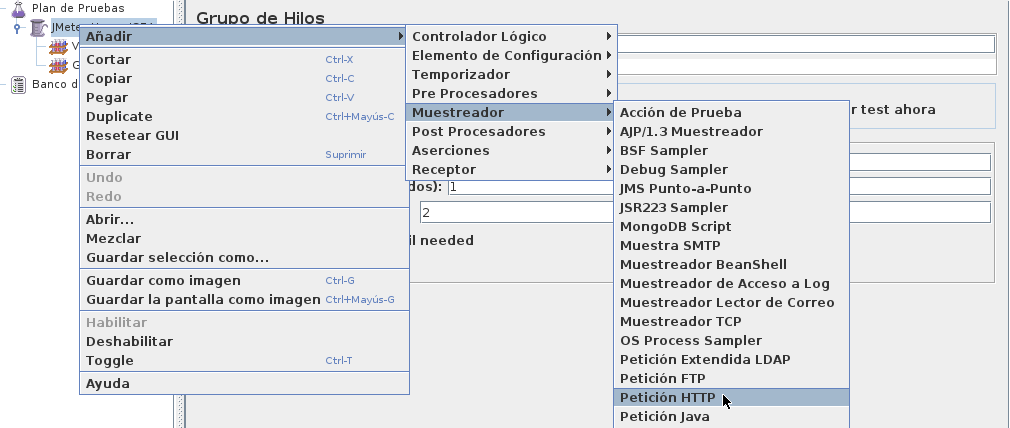
\includegraphics[width=0.5\textwidth]{16}
        \caption{Ruta a seguir para añadir peticiones HTTP a nuestro \textit{test plan}}
        \label{rutapethtt}
    \end{figure}

    \item En la ventana que obtendremos, sólo tenemos que cambiar el nombre de la petición por \textit{Home Page} y establecer la ruta a ``/''. No debemos indicar el nombre del servidor, ya que lo hemos dejado indicado con anterioridad. Debe quedarnos tal y como se ve en la \hyperref[valpethttp]{Figura \ref*{valpethttp}}.

    \begin{figure}[!h]
        \centering
        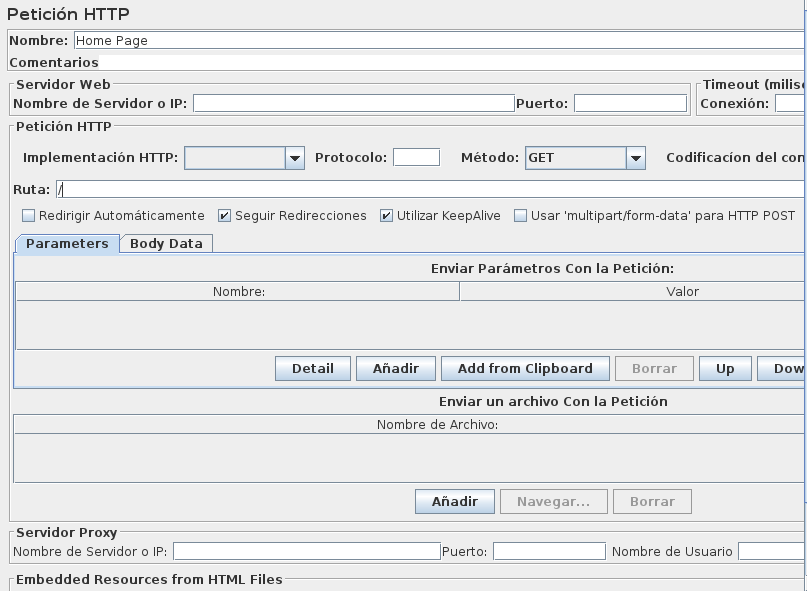
\includegraphics[width=0.5\textwidth]{17}
        \caption{Valores que debe tener nuestra petición HTTP}
        \label{valpethttp}
    \end{figure}

    \item Por último, debemos añadir un \textit{Receptor} para poder guardar los resultados en un fichero y representarlos gráficamente. Para ello, hacemos click derecho en nuestro \textit{Grupo de hilos} y seguimos la ruta \textbf{Añadir $>$ Receptor $>$ Gráfico de Resultados}. (\hyperref[rutareceptor]{Figura \ref*{rutareceptor}}).

    \begin{figure}[!h]
        \centering
        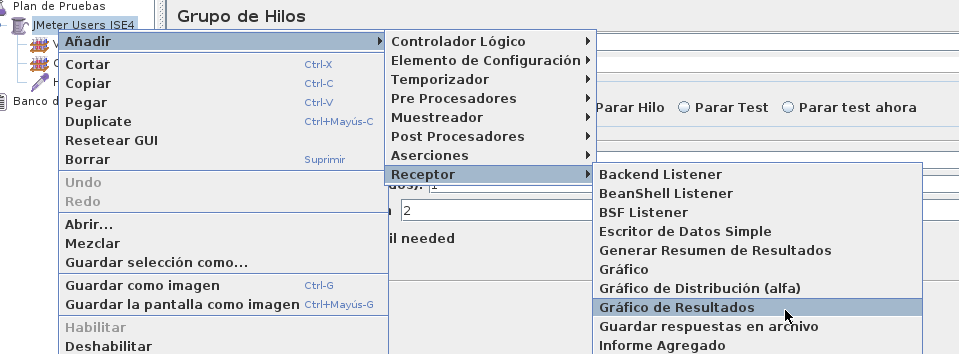
\includegraphics[width=0.5\textwidth]{18}
        \caption{Ruta a seguir para añadir un \textit{Receptor} a nuestro \textit{test plan}}
        \label{rutareceptor}
    \end{figure}

    \item En la ventana que obtendremos, debemos añadir una ruta para guardar los resultados de nuestro \textit{test plan}. Podemos, o bien añadirla escribiendo una ruta, o bien seleccionar la ruta con el botón de Navegar. (\hyperref[ventanareceptor]{Figura \ref*{ventanareceptor}}).

    \begin{figure}[!h]
        \centering
        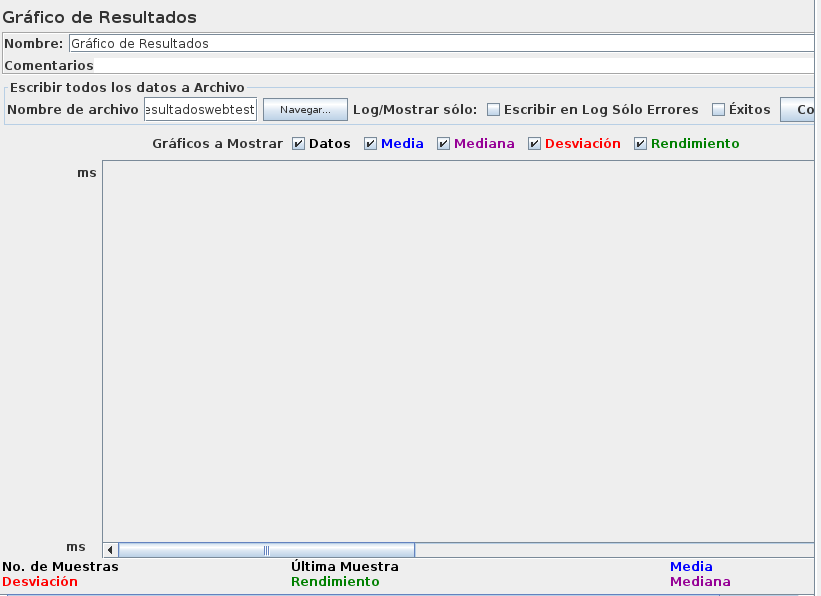
\includegraphics[width=0.5\textwidth]{19}
        \caption{Ventana de configuración del Receptor de nuestro \textit{test plan}}
        \label{ventanareceptor}
    \end{figure}

    \item Guardamos el plan de pruebas que hemos hecho y lo lanzamos siguiendo la ruta \textbf{Lanzar $>$ Arrancar}. Cuando el test finalice, veremos lo resultados reflejados en el gráfico de resultados (\hyperref[graf1]{Figura \ref*{graf1}}). Como sólamente lo ejecutamos dos veces, no obtenemos muchos valores para representar en nuestra gráfica, si cambiamos el parámetro \textit{Contador del bucle} de nuestro \textit{grupo de hilos} a un número mayor, obtendremos más valores para nuestra gráfica (\hyperref[graf2]{Figura \ref*{graf2}}). En los resultados obtenidos, podemos ver cómo conforme se va incrementando el número de peticiones, va aumentando el tiempo de respuesta del servidor.

    \begin{figure}[H]
        \centering
        
        \mbox {
            \subfigure[Gráfico obtenido tras ejecutar nuestro \textit{test plan} dos veces]{
            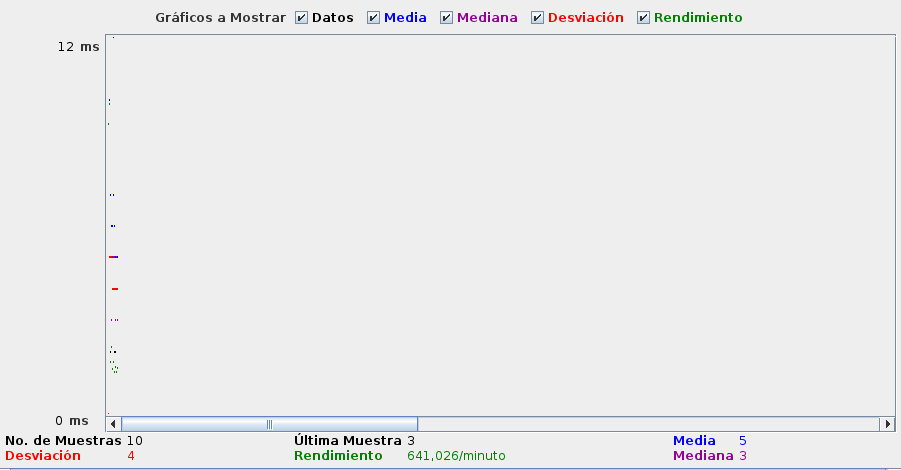
\includegraphics[width=0.55\textwidth]{20}
            \label{graf1}
        }
        \qquad
        
        \subfigure[Gráfico obtenido tras ejecutar nuestro \textit{test plan} 200 veces] {
            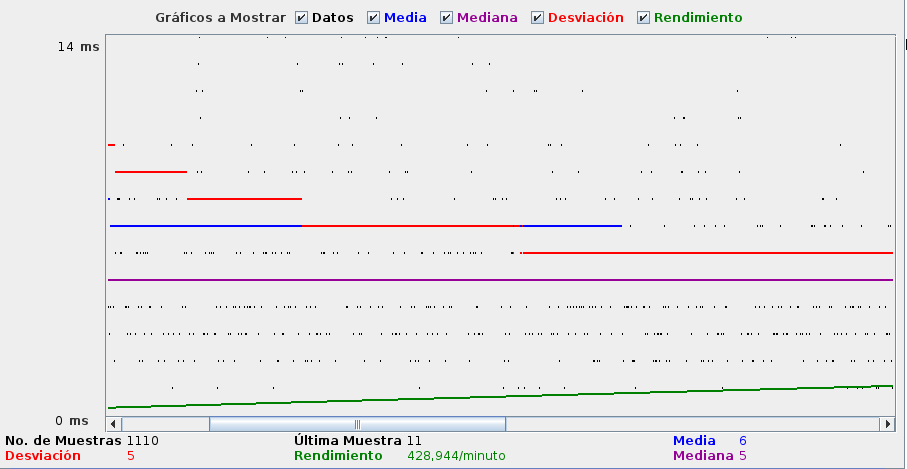
\includegraphics[width=0.55\textwidth]{21}
            \label{graf2}
            }
        }
        \caption{Ejecutando nuestro \textit{test plan}}
        \label{graf}
    \end{figure}
\end{enumerate}

\section{Programe un \textit{benchmark} usando el lenguaje que desee. El \textit{benchmark} debe incluir: 1) Objetivo del \textit{benchmark}, 2) Métricas (unidades, variables, puntuaciones, etc), 3) Instrucciones para su uso y 4) Ejemplo analizando los resultados.}

\subsection{Objetivo del \textit{benchmark}}
El \textit{benchmark} a realizar se trata de un script en \textit{Python} usando \textbf{peewee} (\cite{intropeewee}) para comparar \textit{SQLite} y \textit{MySQL}. En concreto, se medirán los siguientes parámetros:
\begin{enumerate}[$\bullet$]
    % \item Velocidad de acceso a tablas completas de gran tamaño en la base de datos ($V_{grande}$).
    % \item Velocidad de acceso a tablas completas con poco tamaño en la base de datos ($V_{peque}$).
    \item Velocidad para hacer una consulta concreta en una tabla grande ($V_{consultag}$).
    \item Velocidad para hacer una consulta concreta en una tabla pequeña ($V_{consultap}$).
    \item Velocidad para introducir un dato en una tabla pequeña ($V_{escriturap}$).
    \item Velocidad para introducir un dato en una tabla grande ($V_{escriturag}$).
    \item Velocidad para eliminar un dato en una tabla pequeña ($V_{borradop}$).
    \item Velocidad para eliminar un dato en una tabla grande ($V_{borradog}$).
\end{enumerate}

Donde el tamaño de la tabla grande es de 3503 filas y el de la tabla pequeña, 25.

Con estos parámetros, el objetivo de este benchmark es averiguar qué gestor de bases de datos es mejor para alguien que realiza consultas y escrituras de forma habitual en una base de datos.

\subsection{Métricas}
Todos estos parámetros se medirán en \textbf{segundos} y para saber el resultado final se usará un diagrama de barras. Cada parámetro medido aparecerá en el diagrama de barras y se tomará como mejor aquel que haga el trabajo en menor número de segundos.

Para obtener cada parámetro, se hará la misma consulta cuatro veces y se hará la media del tiempo obtenido en cada operación. La primera consulta de todas se despreciará, debido a que la base de datos no se encontrará en cache y será más lenta.

\subsection{Instrucciones de uso}
Para usar el benchmark, sólo debemos ejecutar el script en Python \texttt{benchmarkbd.py} y esperar a que termine su ejecución.

\begin{minted}[frame=single, label={Ejecutando el benchmark}]{bash}
python benchmarkbd.py
\end{minted}

\subsection{Ejemplo de ejecución}
Tras ejecutar el benchmark, obtenemos la gráfica de la \hyperref[benchmarkbasedatos]{Figura \ref*{benchmarkbasedatos}}.

\begin{figure}[!h]
    \centering
    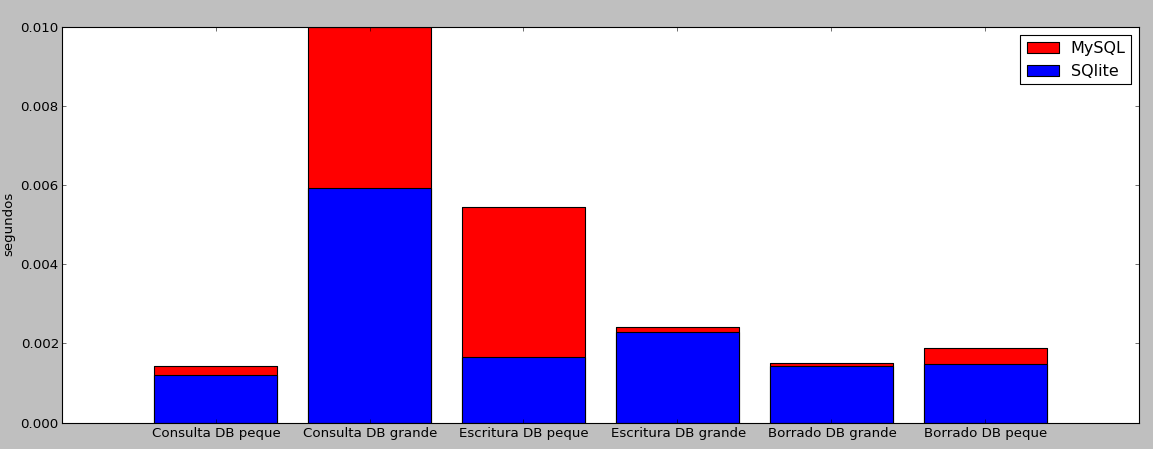
\includegraphics[width=1\textwidth]{22}
    \caption{Resultados tras ejecutar el benchmark}
    \label{benchmarkbasedatos}
\end{figure}

A pesar de que históricamente \textit{SQLite} era más lento que \textit{MySQL} (\cite{speedcom}), en la última versión se ha visto bastante optimizado, llegando a conseguir mejores resultados que \textit{MySQL}. Por tanto, el gestor de base de datos que mejores resultados ha dado es \textit{SQLite}.

\subsection{Detalles sobre el Script}
Para generar los modelos\footnote{En \textit{peewee}, los \textbf{Modelos} representan cada tabla de la base de datos en una clase de Python.} y así poder empezar a hacer consultas debemos ejecutar el siguiente comando:
\begin{minted}[frame=single, label={Creando los modelos de la base de datos}]{bash}
pyhton -m pwiz -e mysql -u root -P Chinook > modelos.py
\end{minted}

El script en Python, cambia de base de datos en tiempo de ejecución. Mas concretamente, cambia de una a otra cuando se han realizado los calculos de la primera:

\mypython[label={benchmarkbd.py}]{benchmarkbd.py}

\section{Cuestiones opcionales}
\subsection{Seleccione, instale y ejecute un benchmark, comente los resultados. \textbf{Atención}: no es lo mismo un benchmark que una suite, instale un benchmark}
En nuestro caso, de toda la lista de benchmarks disponibles, hemos elegido uno para medir la capacidad de la CPU para comprimir video usando la librería \texttt{x264} (\cite{x264}). Para instalarlo, según \cite{phoronixubuntu}, usamos el siguiente comando:
\begin{minted}[frame=single, label={Instalando el benchmark x264}]{bash}
sudo phoronix-test-suite benchmark x264
\end{minted}

tras esto, empezará a descargar e instalar el benchmark y sus dependencias. Una vez instalado nos mostrará el sofware y hardware de nuestra máquina y nos preguntará si queremos guardar la información en un fichero y si le decimos que no, empezará a hacer pruebas. En la prueba que hemos hecho en la \hyperref[x264test]{Figura \ref*{x264test}}, el benchmark nos da como conclusión que podríamos codificar unos 26 \textit{frames} por segundo. 

\begin{figure}[!h]
\centering
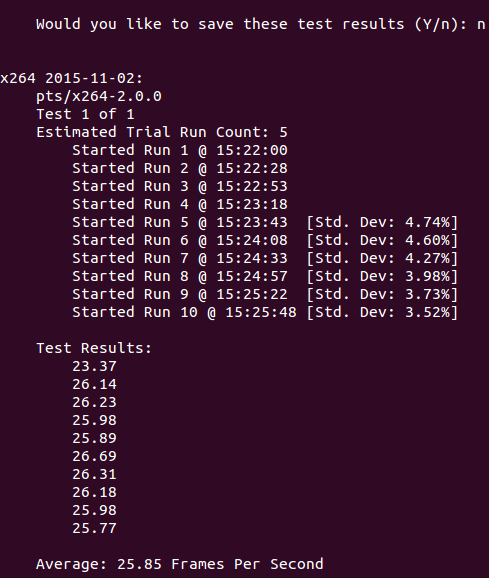
\includegraphics[width=0.5\textwidth]{3}
\caption{Salida del benchmark \texttt{x264} mientras realiza sus pruebas}
\label{x264test}
\end{figure}

\setcounter{subsection}{2}
\subsection{Lea el artículo de comparación entre \textit{Jmeter} y \textit{Gatling} elaborado por la empresa \textit{Flood.io} y elabore un breve resumen}
En \textit{Flood.io} no se fían de los benchmark ``competitivos'' ya que están hechos para favorecer a las empresas que lo patrocinan y no dan resultados realmente fiables. Por eso, se pasaron al lado del código abierto y probaron \textit{Jmeter} y \textit{Gatling}.

Tras hacer el \textit{test plan} con los dos benchmark, en el cual había 10.000 usuarios y 30.000 peticiones por minuto, el resultado obtenido es que ambos benchmark son bastante parecidos pero tienen una diferencia: \textit{Gatling} no es capaz de guardar el tamaño en bytes de la respuesta, pero sin embargo, a pesar de que \textit{Jmeter} sí lo es consume más recursos de CPU y memoria.

El artículo concluye diciendo que ambos benchmark son muy parecidos en términos de concurrencia y \textit{throughput} y que la elección de uno u otro es puramente subjetiva y hecha sobre alguna otra característica que cada herramienta incluya.


\bibliography{P4-MarGomMac.bib} %archivo citas.bib que contiene las entradas 
\bibliographystyle{siam} % haycle varias formas de citar

\end{document}
